MapReduce is a (functional) programming model for processing large amounts of
data over a distributed network of nodes. Probably the most known implementation
of MapReduce is Hadoop \cite{Hadoop}. Data can be manipulated by defining a map
and reduce funtion. A map function transforms data from one form into another
and a reduce function combines multiple data entries into a single entry.
MapReduce essentially works by splitting the potentially huge input data up into
several partitions. Each partition is then sent off to a different worker in the
network, which in turn applies the map function on the data partition. This is
called the map phase. The result of the map operation is usually stored
temporarily on disk. Once all the partitions have been processed by the nodes in
the network, the reduce phase is started. The nodes all read a specific range of
the output from the map phase, and then apply the reduce function on that data.
The resulting data is sent to an output file. An overview is given in figure
\ref{fig:mapreduce}. Once the framework which implements MapReduce has completed
both phases the result can be read. This programming model allows developers to
solve problems quickly while leveraging a cluster of computers, which with a
single computer would take significantly longer. Obviously there is a penalty
for having to use the network, but this is offset by the fact that the
map-reduce cluster is capable of solving problems with very large input sets.

\begin{figure}[htb] 
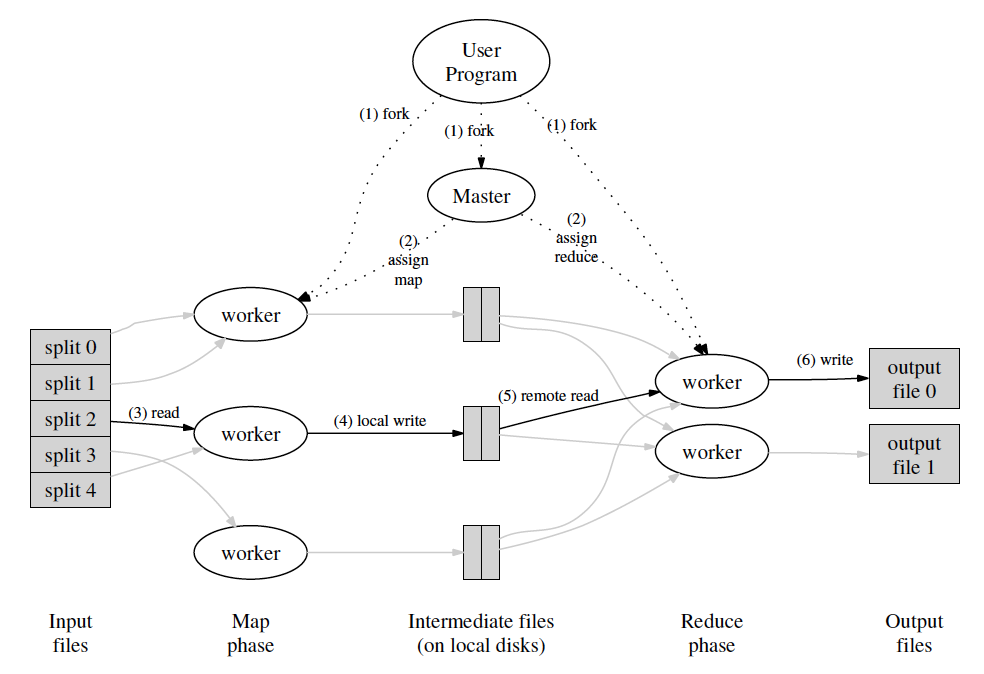
\includegraphics[width=340px]{mapreduce.png} 
\caption{Image from: MapReduce: Simplified Data Processing on Large Clusters, 2004, by Jeffrey Dean and Sanjay Ghemawat} \label{fig:mapreduce} 
\end{figure}
